\chapter{Potentials}

\section{Laplace's Equation}

\subsection{Introduction}

We are interested in the differential form of Poisson's equation,
\[\nabla^2V=-\frac{\rho}{\varepsilon_0},\]
which is equivalent to the integral form
\[V(\vec{r})=\frac{1}{4\pi\varepsilon_0}\iiint\frac{\rho(\vec{r'})}{\scr}d\tau'\]
if we're given boundary conditions.

More often, we're interested in finding the potential in regions where $\rho=0$. Here, Poisson's equation reduces to Laplace's equation
\[\nabla^2V=0,\qquad\text{or}\qquad \frac{\partial^2V}{\partial x^2}+\frac{\partial^2V}{\partial y^2}+\frac{\partial^2V}{\partial z^2}=0.\]
This is so fundamental the subject that one might say electrostatics \textit{is} the study of Laplace's equation. This equation plays a role in many branches of physics and mathematics.

\begin{definition}
A solution to Laplace's equation is called a \vocab{harmonic function}.
\end{definition}

To get a feel for these harmonic functions, we will begin in lower dimensions.

\subsection{Laplace's Equation in One Dimension}

In one dimension, Laplace's equation is
\[\frac{d^2V}{dx^2}=0.\]
This means the derivative $\frac{dV}{dx}$ is constant over $x$; hence, the general solution is a straight line
\[V(x)=mx+b.\]
Since it contains two free variables, this solution is appropriate for a second-order differential equation (as we need to specify some pair of either $V$ or $V'$ as initial conditions).

There are two important features of this result that generalize nontrivially in higher dimensions:
\begin{enumerate}
    \item $V(x)$ is the \textit{average} of $V(x+a)$ and $V(x-a)$, for \textit{any} $a$:
    \[V(x)=\frac{1}{2}[V(x+a)+V(x-a)].\]
    Hence, Laplace's equation tells you to average values; if you're given some endpoints as boundary conditions, harmonic functions are, in this sense, as \textit{boring as they possibly could be} yet still fit the endpoints.
    \item Laplace's equation allows \textit{no local maxima or minima}; the only extreme values of $V$ can occur at the endpoints. This is a consequence of the above property: if there were a local maxima then it wouldn't be an average of its neighbors.
\end{enumerate}

\subsection{Laplace's Equation in Two Dimension}

In two dimensions, Laplace's equation is
\[\frac{\partial^2V}{\partial x^2}+\frac{\partial^2V}{\partial y^2}=0.\]
This is no longer an ordinary differential equation: the partial derivatives make it a \textit{partial} differential equation. Thus, some simple rules no longer apply: for example, the general solution doesn't contain two free variables (or any finite number of free variables) even though it is second order. Therefore, one cannot write down a simple ``general solution", at least not in closed form.

An example of a two-dimensional harmonic function is obtained by stretching a thin rubber sheet (or a soap film) over a support. Then, the resultant function will be roughly a harmonic function. These have the same two properties that we saw in one dimension:

\begin{enumerate}
    \item The value of $V$ at a point $(x,y)$ is the average of those \textit{around} the point: more precisely, if you draw a circle of any radius $R$ about the point $(x,y)$, then 
    \[V(x,y)=\frac{1}{2\pi R}\oint_{\text{circle}}Vd\ell.\]
    This suggests the \vocab{method of relaxation} for solving Laplace's equation given boundary conditions, which involves starting with a reasonable set of guesses then iteratively refining the guesses by averaging out points until they settle.
    \item $V$ has no local maxima or minima; all extrema occur at the boundaries. Once again, this follows from the previous property.
\end{enumerate}

\subsection{Laplace's Equation in Three Dimensions}

Now we're onto the good stuff. However, now we can offer neither an explicit solution nor a suggestive physical example. Nonetheless, the same two properties hold, and a proof will be sketched (using Coulomb's law; a proof using only Laplace's equation is given as a problem at the end of the chapter).

\begin{proposition}
The two properties hold for harmonic functions in three dimensions:
\begin{enumerate}
    \item The value of $V$ at a point $\vec{r}$ is the average of $V$ over a spherical surface of radius $R$ centered at $\vec{r}$:
    \[V(\vec{r})=\frac{1}{4\pi R^2}\oiint_{\text{sphere}}V da.\]
    \item Hence, $V$ has no local maxima or minima; the extrema must occur at boundaries.
\end{enumerate}
\end{proposition}

\begin{proof}
Let's calculate the average potential over a spherical surface of radius $R$ due to a \textit{single} point charge $q$ located outside the sphere. Place the sphere at the origin, and put $q$ on the $z$-axis, $z$ away from the center of the sphere.

Then, we can calculate the average potential across the sphere to be
\begin{align*}
    \frac{1}{4\pi R^2}\oiint_{\text{sphere}}Vda&=\frac{1}{4\pi R^2}\int_{\varphi=0}^{2\pi}\int_{\theta=0}^\pi \frac{1}{4\pi\varepsilon_0}\frac{q}{\sqrt{z^2+R^2-2zR\cos\theta}}R^2\sin\theta d\theta d\varphi\\
    &=\frac{q}{8\pi \varepsilon_0}\int_0^\pi \frac{\sin\theta}{\sqrt{z^2+R^2-2zR\cos\theta}}d\theta\\
    &=\frac{q}{8\pi\varepsilon_0}\left[-\frac{1}{zR}\cdot \sqrt{z^2+R^2-2zR\cos\theta}\right]_0^\pi\\
    &=\frac{q}{8\pi\varepsilon_0zR}\left(\sqrt{z^2+R^2-2zR}-\sqrt{z^2+R^2+2zR}\right)\\
    &=\frac{q}{4\pi\varepsilon_0z},
\end{align*}
which is exactly the electric potential at the center! By the superposition principle, the same goes for \textit{any collection} of charges outside the sphere: their average potential over the sphere is equal to the net potential they produce at the center. Note that we ignore cases where there are charges inside the sphere, since that would violate $\rho=0$.
\end{proof}

\subsection{Boundary Conditions and Uniqueness Theorems}\label{boundconduniqthm}

Laplace's equation by itself doesn't determine $V$; we need boundary conditions. But what boundary conditions are appropriate to restrict $V$ sufficiently but not cause inconsistencies?

It is clear in one dimension, but the \textit{partial} differential equations in two and three dimensions make the issue harder.  As it turns out, $V$ \textit{is} uniquely determined by its value at the boundary. However, other boundary conditions can also be used. The proof that a proposed set of boundary conditions will suffices is usually presented in the form of a \vocab{uniqueness theorem}; we do not seek to prove the \textit{existence} of solutions, but this is generally clear on physical grounds.

\begin{theorem}[First uniqueness theorem]
    The solution to Laplace's equation in some volume $\mathcal{V}$ is uniquely determined if $V$ is specified on the boundary surface $\partial\mathcal{V}$.
\end{theorem}

\begin{proof}
There is a rather clever trick to solve this problem: suppose that there exist two such solutions $V_1$ and $V_2$ such that $V_1=V_2$ on $\partial\mathcal{V}$ and $\nabla^2 V_1=\nabla^2 V_2=0$ inside $\mathcal{V}$.

The key is to \textbf{consider the difference} $V_3:=V_1-V_2$. Now, $V_3=0$ on all of $\partial \mathcal{V}$, and because of the linearity of the del operator, we have
\[\nabla^2V_3=\nabla^2 V_1-\nabla^2V_2=0\]
inside all of $\mathcal{V}$; hence $V_3$ is also a harmonic function. However, $V_3$ has no local extrema inside $\mathcal{V}$, and since it is zero on all of $\partial\mathcal{V}$, this implies that it is indeed zero inside all of $\mathcal{V}$ as well (otherwise we would be able to find some local extrema not at the boundary). Hence $V_1=V_2$, and the solution is unique.
\end{proof}

\begin{example}
Show that the potential is \textit{constant} inside an enclosure completely surrounded by conducting material, provided there is no charge within the enclosure.
\end{example}

\begin{proof}
Since it is a conductor, the boundary of the enclosure is equipotential, say at $V_0$. It is easy to see that $V=V_0$ everywhere inside is a valid solution to Laplace's equation. The first uniqueness theorem guarantees that this is the only one.
\end{proof}

It turns out the first uniqueness theorem works even if we sprinkle in some charge: the argument works the same, instead now we subtract $\nabla^2V_1=\nabla^2V_2=-\frac{\rho}{\varepsilon_0}$ to get $\nabla^2V_3=0$. In either case, the \textit{difference} $V_3:=V_1-V_2$ is a harmonic function and hence satisfies Laplace's equation with zeros on the boundary.

\begin{corollary}
The potential in a volume $\mathcal{V}$ is uniquely determined if we specify  
\begin{enumerate}[(a)]
    \item the charge density throughout the region and
    \item the values of $V$ on all boundaries.
\end{enumerate}
\end{corollary}

\subsection{Conductors and the Second Uniqueness Theorem}

If we don't know the potentials of certain conductors (by attaching them to the zero potential ground or fixed potential batteries) and instead we know the charges on conductors, do we know that there exists one unique charge distribution and therefore generated electric field? As it turns out, we do.

\begin{theorem}[Second uniqueness theorem]
    In a volume $\mathcal{V}$ surrounded by conductors and containing a specified charge density $\rho$, the electric field is uniquely determined if the \textit{total} charge on each conductor is given. (The outer boundary can be at infinity, so unbounded.)
\end{theorem}

\begin{proof}
    Once again, assume there exist two electric fields $\vec{E}_1$ and $\vec{E}_2$. We know that in the space between the conductors,
    \[\nabla\cdot \vec{E}_1=\nabla\cdot\vec{E}_2=\frac{\rho}{\varepsilon_0}.\]
    In addition, for a Gaussian surface $\mathcal{S}_i$ just enclosing the $i$th conductor with charge $Q_i$, we have that
    \[\oiint_{\mathcal{S}_i}\vec{E}_1\cdot d\vec{a}=\oiint_{\mathcal{S}_i}\vec{E}_2\cdot d\vec{a}=\frac{Q_i}{\varepsilon_0}.\]
    In addition, if we set the Gaussian surface as the outer boundary, we get
    \[\oiint_{\text{outer boundary}}=\vec{E}_1\cdot d\vec{a}=\oiint_{\text{outer boundary}}=\vec{E}_2\cdot d\vec{a}=\frac{Q_{\text{tot}}}{\varepsilon_0}.\]
    Now, we examine the difference $\vec{E}_3:=\vec{E}_1-\vec{E}_2$, which obeys 
    \[\nabla\cdot \vec{E}_3=0\]
    in the region between conductors, and
    \[\oiint\vec{E}_3\cdot d\vec{a}=0\]
    over each of the bounding surfaces $\mathcal{S}_i$ as well as the outer boundary.
    
    Finally, we exploit the fact that each conductor is an equipotential; hence $V_3$ is \textit{constant} over each conducting surface (not necessarily the same constant across different conductors). Then, invoking one of the divergence product rules (in Theorem \ref{divprodrul}), we get
    \[\nabla\cdot (V_3\vec{E}_3)=V_3(\nabla\cdot \vec{E}_3)+\vec{E}_3\cdot(\nabla V_3)=-(E_3)^2,\]
    where we use that $\nabla\cdot\vec{E}_3=0$ and $\vec{E}_3=-\nabla V_3$. Now, we integrate this over $\mathcal{V}$, the space inside the outer boundary between all the conductors, and apply the divergence theorem to get
    \[-\iiint_{\mathcal{V}}(E_3)^2d\tau=\iiint_{\mathcal{V}}\nabla\cdot(V_3\vec{E}_3)d\tau=\oiint_{\partial\mathcal{V}}V_3\vec{E}_3\cdot d\vec{a}=V_3\cdot\oiint_{\partial\mathcal{V}}\vec{E}_3\cdot d\vec{a}=0.\]
    as 
    \[\partial\mathcal{V}=\text{(outer boundary)}\cup \left(\bigcup_i\mathcal{S}_i\right),\]
    so $V_3$ is constant on all these surfaces; further, the remaining integral of $\vec{E}_3$ is also zero on each of these surfaces.
    
    However, the integrand $(E_3)^2$ on the left hand side is nonnegative, so the only way for the whole integral to equal zero is if $|\vec{E}_3|=0$ everywhere. Hence, $\vec{E}_1=\vec{E}_2$, as desired.
\end{proof}

This proof is not easy, and the theorem is not as obvious as you might think. 

\begin{example}
Consider the setup below on the left, with four charges arranged as shown. Now, use a pair of conducting wires to connect pairs of charges. This setup seems reasonable: the positive and negative charges are near each other, which is where they like to be. However, the setup is actually \textit{impossible}; use the second uniqueness theorem to prove this.
\end{example}

\begin{center}
    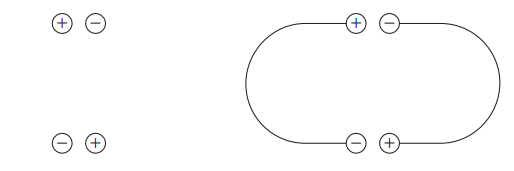
\includegraphics[width=8cm]{Electrodynamics/images/fig3.7-8.PNG}
\end{center}

\begin{proof}
Why will current flow? Well, we have a situation where the \textit{total} charge on each conductor is zero; therefore, there should be a unique way of distributing the charges across each conductor that generate the external electric field. \textit{One} way of doing so involves simply making the charge zero everywhere in each conductor. By the second uniqueness theorem we just proved, this is the \textit{only} way! So the charge will flow along the wires, canceling off.
\end{proof}

\section{The Method of Images}

\subsection{The Classic Image Problem}

It's time to present an incredible trick; it will almost feel like cheating.

\begin{example}
Suppose a point charge $q$ is held a distance $d$ above an infinite grounded conducting plane. What is the potential in the region above the plane?
\end{example}

\begin{proof}
First, note that the answer isn't simply $\frac{1}{4\pi\varepsilon_0}\frac{q}{\scr}$; the conducting plane actually does something since the electric field induces some negative charge on the nearby surface of the conductor, which affects the potential.

But how can we possibly determine the potential, if we don't know how much charge is induced or how it is distributed?

Let's place the infinite grounded conducting plane in the $xy$-plane, and the point charge at $(0,0,d)$ along the $z$-axis. Now, the problem is to solve Poisson's equation in the half-plane $z>0$ with a single point charge $q$ at $(0,0,d)$, subject to the boundary conditions
\begin{enumerate}
    \item $V=0$ when $z=0$ (as the conducting plane is grounded),
    \item $V\to 0$ at infinity.
\end{enumerate}
The first uniqueness theorem guarantees that there is a unique function $V$ that satisfies these boundary conditions. How can we construct such a function?

Here's the trick: consider a completely different setup, which consists of a point charge $q$ at $(0,0,d)$ and a point charge $-q$ at $(0,0,-d)$. The key point is that the half-plane $z>0$ has the same charge distribution, and the boundary conditions still hold:
\begin{enumerate}
    \item $V=0$ when $z=0$,
    \item $V\to 0$ at infinity.
\end{enumerate}
This is because the symmetric placement of a $-q$ charge ensures that the electric potential cancels along $z=0$. Therefore, the solution to $V$ in this setup, by the first uniqueness theorem, \textit{is the same} as the solution to $V$ in the first setup. Hence, the answer is
\[V(x,y,z)=\frac{q}{4\pi\varepsilon_0}\left[\frac{1}{\sqrt{x^2+y^2+(z-d)^2}}-\frac{1}{\sqrt{x^2+y^2+(z+d)^2}}\right] \qquad (z\ge 0).\]
The ``lower region" $z<0$ is still completely different, and we do not understand it using this method.
\end{proof}

\subsection{Induced Surface Charge}

\begin{example}
In the setup above, determine the surface charge $\sigma$ induced on the conductor.
\end{example}

\begin{proof}
In the most general situation, we can simply invoke the equation
\[\frac{\partial V}{\partial n}=-\frac{\sigma}{\varepsilon_0}\]
from Subsection \ref{surfcharforcond}, where $\frac{\partial V}{\partial n}=(\nabla V)\cdot\hat{n}$ is the directional derivative in the normal direction.

In the situation above, we can take
\begin{align*}
\sigma(x,y)&=-\varepsilon_0\left.\frac{\partial V}{\partial z}\right\rvert_{z=0}\\
&=-\varepsilon_0\cdot \frac{q}{4\pi\varepsilon_0}\left[\frac{d-z}{(x^2+y^2+(z-d)^2)^{3/2}}+\frac{d+z}{(x^2+y^2+(z+d)^2)^{3/2}}\right]_{z=0}\\
&=\boxed{\frac{-qd}{2\pi(x^2+y^2+d^2)^{3/2}}}.
\end{align*}
For some sanity checks, note that the induced charge is negative and greatest at $x=y=0$. For a further sanity check, we can integrate it over the plane
\begin{align*}
    \iint_{\mathbb{R}^2}\sigma(x,y)da&=\int_{\theta=0}^{2\pi}\int_{r=0}^\infty \frac{-qd}{2\pi(r^2+d^2)^{3/2}}\cdot rdrd\theta\\
    &=-q\int_{0}^\infty\frac{rd}{(r^2+d^2)^{3/2}}dr\\
    &=-q\left[\frac{d}{2}\cdot \frac{-2}{\sqrt{r^2+d^2}}\right]_0^\infty=-q,
\end{align*}
as expected.

\end{proof}

\subsection{Force and Energy}

\begin{example}
What is the force of attraction between the point charge and the plane?
\end{example}

\begin{proof}
Once again, considering the analog problem with two point charges $+q$ and $-q$ suffices, since the local potential around $+q$ is all that determines the force on it, and it is the same in both setups. Therefore, the force is simply
\[\vec{F}=-\frac{1}{4\pi\varepsilon_0}\frac{q^2}{(2d)^2}\hat{z}.\]
\end{proof}

\begin{example}
How do the energies of the two analogous setups (the point charge and plane versus the two opposite point charges) compare?
\end{example}

\begin{proof}
With two point charges, the energy is simply
\[W=-\frac{1}{4\pi\varepsilon_0}\frac{q^2}{2d}.\]
However, it turns out that for a single charge and conducting plane, the energy is \textit{half}:
\[W=-\frac{1}{4\pi\varepsilon_0}\frac{q^2}{4d}.\]
One way to figure out why is to consider the energy stored in the fields
\[W=\iiint_{\mathbb{R}^3}\frac{\varepsilon_0E^2}{2}d\tau,\]
and note that in the plane case we only have the upper region $z\ge 0$ of fields, so we should only get half the energy.

We can also compute the energy by calculating the work required to bring $q$ in from infinity.
\end{proof}

\begin{remark}
One way to conceptualize the difference between these cases is that with the plane,w e are doing work on a \textit{single} point charge to bring it in. The induced charge on the conductor is shifting around, but this costs no work since the potential is zero (you can also think of the fact that it is a conductor, so charge can move around freely).

In the analog case with two charges, however, we need to do work to pull in \textit{both} of them, so the energy stored is twice as much.
\end{remark}

\subsection{Other Image Problems}

We can apply the above technique to any collection of point charges near a grounded conducting plane by introducing the mirror image of the setup with opposite charges (notice how introducing these opposite charges ensures that the potential along where the plane should be is 0). We call this the \vocab{method of images}.

The following application of the method of images is beautiful, and relates to circle (sphere) inversion and Apollonius circles (spheres).

\begin{example}
A point charge $q$ is situated a distance $a$ from the center of a grounded conducting sphere of radius $R$. Find the potential outside the sphere.
\end{example}

\begin{proof}
\textit{Invert} (!!) the point charge $q$ about the sphere; this gives a point that is a distance 
\[b=\frac{R^2}{a}\]
away from the center, along the ray from the center of the sphere to the point charge $q$. Imbue this point charge with charge
\[q'=-\frac{R}{a}q.\]
We claim that this setup has zero potential along the surface of the sphere; this is true by Appolonius spheres. Therefore, the potential is indeed
\[\boxed{V(\vec{r})=\frac{1}{4\pi\varepsilon_0}\left(\frac{q}{\scr}+\frac{q'}{\scr'}\right)}\]
outside the sphere, where $\scr$ is the distance to $q$ and $\scr'$ is the distance to $q'$.
\end{proof}

\begin{remark}
You cannot place image charges in the region where you are calculating $V$! That would charge $\rho$, and you'd be solving Poisson's equation with incorrect $\rho$ (even if the boundary conditions are the same).
\end{remark}

\begin{example}
What is the force of attraction between the point and sphere?
\end{example}

\begin{proof}
It is simply the force between the charge and the image charge $q'$ we placed:
\[F=\frac{1}{4\pi\varepsilon_0}\frac{qq'}{(a-b)^2}=\boxed{-\frac{1}{4\pi\varepsilon_0}\frac{q^2Ra}{(a^2-R^2)^2}}.\]
\end{proof}

The method of images is incredibly simple and magical. It comes down to figuring out the correct ``auxiliary" configuration of image charges to make sure the grounded conductors in the setup have potential zero. However, for most shapes, this is forbiddingly complicated, if not impossible. So use with care!

\section{Separation of Variables}

Recall that in Section \ref{boundconduniqthm} we proved the first uniqueness theorem, which states that if $V$ is given on a boundary $\partial\mathcal{V}$, then it is uniquely determined on the interior of the volume, and therefore the entire volume $\mathcal{V}$. This is because $V$ satisfies Laplace's equation $\nabla^2 V=0$ (assuming there is no charge distribution in the volume).

In this section, we try to solve this problem exactly, mathematically. We use a technique called \vocab{separation of variables}. We'll develop the method through a sequence of examples in various coordinate systems.

\subsection{Cartesian Coordinates}

\begin{example}
Two infinite grounded metal plates lie parallel to the $xz$ plane, one at $y=0$, the other at $y=a$. The left end, at $x=0$, is closed off with an infinite strip insulated from the two plates, and maintained at a specific potential $V_0(y)$. Find the potential inside this ``slot."
\end{example}

\begin{center}
    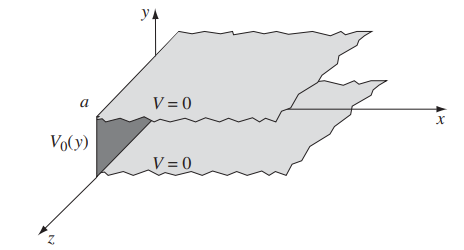
\includegraphics[width=8cm]{Electrodynamics/images/fig3.17.PNG}
\end{center}

\begin{remark}
For an actual physical example of how such a situation could occur, consider placing an infinite charged wire parallel to the $z$ axis at $y=a/2$ and $x=0$, between the two parallel grounded metal plates. This generates some potential along the infinite strip along the $yz$ plane. It also generates some potential in the rest of the volume, but this is the point: our goal is to compute the potential in the slot given the potential along the boundary.
\end{remark}

\begin{proof}
Our goal is to use Laplace's equation $\nabla^2V=0$ to get $V$ in the interior. Note that $V_0(y)$ doesn't depend on $z$, so this is really a $2$-dimensional problem:
\[\frac{\partial^2V}{\partial x^2}+\frac{\partial^2V}{\partial y^2}=0.\]
We are subject to the following boundary conditions:
\begin{enumerate}[(i)]
    \item $V=0$ when $y=0$,
    \item $V=0$ when $y=a$,
    \item $V=V_0(y)$ when $x=0$,
    \item $V\to 0$ when $x\to\infty$.
\end{enumerate}
Since we have $V$ on all the boundaries, by the first uniqueness theorem, it should be uniquely determined within the slot.

Here's the leap: we will start by only investigating solutions $V(x,y)$ to $\nabla^2V=0$ such that it can be expressed as a product of a function depending \textit{only} on $x$ and a function depending \textit{only} on $y$:
\[V(x,y)=X(x)Y(y).\]
This is an \textit{absurd} restriction; we cannot expect $V$ to actually satisfy this! Even something as simple as $V(x,y)=5x+6y$ cannot be written in this form.

However, it turns out that magically, the solutions we \textit{do} get are very special, and pasting them together through linear combinations allows us to construct the general solution. After all, if functions $V_i$ satisfy $\nabla^2 V_i=0$ for all $i$ then so do any linear combinations:
\[\nabla^2\left(\sum_ic_iV_i\right)=\sum_{i}c_i\nabla^2(V_i)=0.\]

Plugging $V(x,y)=X(x)Y(y)$ into $\nabla^2 V=0$ gives
\[\frac{d^2X}{dx^2}Y+X\frac{d^2Y}{dy^2}=0\implies \frac{1}{X}\frac{d^2X}{dx^2}+\frac{1}{Y}\frac{d^2Y}{dy^2}=0.\]
Since these terms are independent (one depends only on $x$ and the other depends only on $y$), they must both be constant. Due to the boundary conditions (this will be clear later), we require that $\frac{1}{X}\frac{d^2X}{dx^2}$ be the positive term. Therefore, we can let
\[\frac{d^2X}{dx^2}=k^2X, \qquad \frac{d^2Y}{dy^2}=k^2Y.\]
These are easy to solve by standard ordinary differential equations methods:
\[X(x)=Ae^{kx}+Be^{-kx}, \qquad Y(y)=C\sin(ky)+D\cos(ky).\]
Hence,
\[V(x,y)=(Ae^{kx}+Be^{-kx})(C\sin(ky)+D\cos(ky)).\]
Now, we need to satisfy the boundary conditions. Boundary condition (iv) requires that $A=0$. Further, boundary condition (i) requires that $D=0$. Finally, (ii) requires that $\sin(ka)=0\implies k=\frac{n\pi}{a}$ for $n\in \NN$. 

That is as far as we can go; unless $V_0(y)$ is some multiple of $\sin\left(\frac{n\pi y}{a}\right)$, we cannot simply fit to (iii). However, it turns out that we can use linear combinations to do so. Patching together our separable solutions allows us to construct much more general functions:
\[V(x,y)=\sum_{n=1}^\infty C_ne^{-n\pi x/a}\sin(n \pi y/a).\]
Now, the goal is to fit
\[V_0(y)=V(0,y)=\sum_{n=1}^\infty C_n\sin(n\pi y/a).\]
This is a \vocab{Fourier sine series}, which by Dirichlet's theorem, is guaranteed to be able to match virtually \textit{any} function $V_0(y)$---even if it has a finite number of discontinuities.

To determine the coefficients, we can use \vocab{Fourier's trick} (which Euler seems to have developed earlier):
\[\int_0^aV_0(y)\sin(n'\pi y/a)dy=\sum_{n=1}^\infty C_n\int_0^a\sin(n\pi y/a)\sin(n'\pi y/a)dy.\]
Now, we can compute that
\[\int_0^a \sin(n\pi y/a)\sin (n'\pi y/a)dy=\begin{cases}
0, & \text{if }n'\neq n,\\
\frac{a}{2}, & \text{if }n'=n.
\end{cases}\]
Hence, extracting the coefficients just amounts to
\[C_n=\frac{2}{a}\int_0^aV_0(y)\sin(n\pi y/a)dy.\]
And we are done:
\[\boxed{V(x,y)=\frac{2}{a}\sum_{n=1}^\infty \left(\int_0^a V_0(y)\sin(n\pi y/a)dy\right)e^{-n\pi x/a}\sin(n\pi y/a)}.\]
\end{proof}

\begin{remark}\label{fixedpot}
For a concrete example, suppose $V_0(y)=V_0$ is a fixed potential. Then,
\[C_n=\frac{2V_0}{a}\int_0^a\sin(n\pi y/a)dy=\frac{2V_0}{n\pi}(1-\cos(n\pi))=\begin{cases}
0, & \text{if }2\mid n,\\
\frac{4V_0}{n\pi} & \text{otherwise}.
\end{cases}\]
Hence, 
\[V(x,y)=\frac{4V_0}{\pi}\sum_{n\text{ odd}}\frac{1}{n}e^{-n\pi x/a}\sin(n\pi y/a)=\frac{2V_0}{\pi}\tan^{-1}\left(\frac{\sin(\pi y/a)}{\sinh (\pi x/a)}\right).\]
Below is a picture of such a potential.
\end{remark}

\begin{center}
    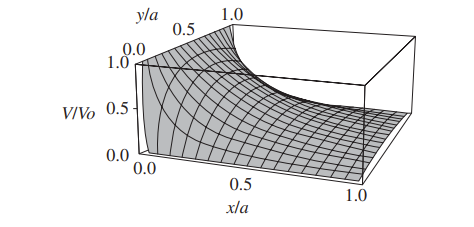
\includegraphics[width=8cm]{Electrodynamics/images/fig3.18.PNG}
\end{center}

This technique is very beautiful, and the mathematics behind it underlines the \vocab{Fourier transform}. If you know some linear algebra, there's a pretty nice way to understand what just happened.

We can consider the vector space of all functions on the interval $[0,a]$; then, we equip the space with an inner product given by
\[\langle f,g\rangle = \frac{2}{a}\int_0^af(y)\ol{g(y)}\cdot dy.\]
However, since $f,g$ are real functions, the complex conjugate doesn't matter. It turns out that this turns the vector space into a \vocab{Hilbert space}; the distance function
\[||f-g||=\sqrt{\langle f-g, f-g\rangle}\]
defined by the inner product makes it a complete metric space (all Cauchy sequences converge). You can check that $||f-g||$ behaves as your intuition would suggest (and therefore our inner product is a good choice): if $f$ and $g$ don't differ much, then $\langle f-g,f-g\rangle$ is small. Now, here's the big claim:

\begin{claim}
The set of functions 
\[\mathcal{B}=\left\{e_n:=\sin\left(\frac{n\pi y}{a}\right):n\in \NN\right\}\]
forms an orthonormal basis of this Hilbert space.
\end{claim}

\begin{proof}
The main point is checking orthogonality: we can do so by just taking inner products:
\begin{align*}
\langle e_m,e_n\rangle &= \frac{2}{a}\int_0^a \sin\left(\frac{m\pi y}{a}\right)\sin\left(\frac{n\pi y}{a}\right)dy\\
&=\frac{1}{a}\int_0^a\left[\cos\left(\frac{(m-n)\pi y}{a}\right)-\cos\left(\frac{(m+n)\pi y}{a}\right)\right]dy=0
\end{align*}
when $m\neq n$. However, if $m=n$, we instead have that it is equal to $1$.

Therefore, $\mathcal{B}$ are indeed orthonormal. Checking that they are spanning as a basis is harder and outside the scope of this text.
\end{proof}

Now, the motivation for Fourier's trick is very clear. If we express any function $f$ in $[0,a]^*$ as a linear combination of vectors in $\mathcal{B}$, we get
\[f=\sum_{n=1}^\infty c_ne_n.\]
Yet in linear algebra, if we ever have a vector written as a linear combination of orthonormal basis vectors in a vector space, how do we extract the coefficients $c_n$? Well, we take the inner product of $f$ with a given basis vector $e_{n'}$:
\begin{align*}
\langle f,e_{n'}\rangle&=\left\langle \sum_{n=1}^\infty c_ne_n, e_{n'}\right\rangle\\
&=\sum_{n=1}^\infty c_n\langle e_n, e_{n'}\rangle\\
&=c_n,
\end{align*}
by linearity of the inner product and the fact that $\langle e_n, e_{n'}\rangle$ equals $0$ when $n\neq n'$ and $1$ when $n=n'$ (orthonormal basis). Therefore,
\[c_n=\langle f,e_n\rangle = \frac{2}{a}\int_0^af(y)\sin(n\pi y/a)dy,\]
as shown before.

\begin{remark}
This linear algebra is really the same computations as the proof of the theorem, but I just find it a nicer way to frame the whole Fourier transform argument.
\end{remark}

Let's do some more examples!

\begin{example}
Two infinitely-long grounded metal plates, again at $y = 0$ and $y = a$, are connected at $x = \pm b$ by metal strips maintained at a constant potential $V_0$, as shown below (a thin layer of insulation at each corner prevents them from shorting out). Find the potential inside the resulting rectangular pipe.
\end{example}

\begin{center}
    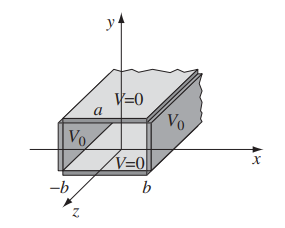
\includegraphics[width=8cm]{Electrodynamics/images/fig3.20.PNG}
\end{center}

\begin{proof}
Once again, the setup doesn't depend on the $z$-coordinate, so it's really a 2-dimensional problem
\[\frac{\partial^2V}{\partial x^2}+\frac{\partial^2V}{\partial y^2}=0\]
under boundary conditions
\begin{enumerate}[(i)]
    \item $V=0$ when $y=0$,
    \item $V=0$ when $y=a$,
    \item $V=V_0$ when $x=-b$,
    \item $V=V_0$ when $x=+b$.
\end{enumerate}
Once again, we search for \textit{separable} functions
\[V(x,y)=X(x)Y(y)\implies \frac{1}{X}\frac{d^2X}{dx^2}+\frac{1}{Y}\frac{d^2Y}{dy^2}=0.\]
Once again, both these terms must be constant:
\[\frac{d^2X}{dx^2}=k^2X, \qquad \frac{d^2Y}{dy^2}=-k^2Y.\]
Solving gives
\[X(x)=Ae^{kx}+Be^{-kx}, \qquad Y(y)=C\sin(kx)+D\cos(kx).\]
Since $V(x,y)=V(-x,y)$, we have $A=B$, so we can write
\[V(x,y)=\cosh (kx)(C\sin (ky)+D\cos (ky)).\]
Further, boundary conditions (i) and (ii) gives $D=0$ and $k=n\pi /a$. Thus,
\[V(x,y)=C\cosh(n\pi x/a)\sin(n\pi y/a).\]
Now, we need to match boundary condition (iii) (note that (iv) follows immediately from the even-ness in $x$).

To do so, let's use a linear combination
\[V(x,y)=\sum_{n=1}^\infty C_n
\cosh(n\pi x/a)\sin(n\pi y/a).\]
Now, we require that
\[V_0=V(b,y)=\sum_{n=1}^\infty \left(C_n\cosh (n\pi b/a)\right)\sin(n\pi y/a).\]
From Remark \ref{fixedpot}, this implies
\[C_n\cosh(n\pi b/a)=\begin{cases}
0, & \text{if }2\mid n,\\
1, & \text{otherwise}.
\end{cases}\]
Finally, the potential in this case is
\[\boxed{V(x,y)=\frac{4V_0}{\pi}\sum_{n\text{ odd}}\frac{1}{n}\frac{\cosh(n\pi x/a)}{\cosh(n\pi b/a)}\sin(n\pi y/a)}\]
\end{proof}

\begin{example}
An infinitely long rectangular metal pipe (sides $a$ and $b$) is grounded, but one end, at $x = 0$, is maintained at a specified potential $V_0(y,z)$, as indicated in the figure below. Find the potential inside the pipe.
\end{example}

\begin{center}
    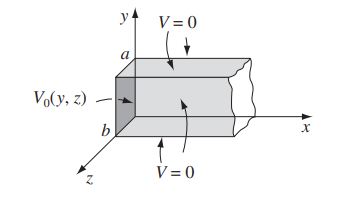
\includegraphics[width=8cm]{Electrodynamics/images/fig3.22.PNG}
\end{center}

\begin{proof}
Now we have a truly three-dimensional problem. We need to solve
\[\frac{\partial^2V}{\partial x}+\frac{\partial^2V}{\partial y}+\frac{\partial^2V}{\partial z}=0\]
under boundary conditions
\begin{enumerate}[(i)]
    \item $V=0$ when $y=0$ or $y=a$,
    \item $V=0$ when $z=0$ or $z=b$,
    \item $V\to 0$ when $x\to \infty$,
    \item $V=V_0(y,z)$ when $x=0$.
\end{enumerate}
As before, we consider separable $V(x,y,z)=X(x)Y(y)Z(z)$ and note that
\[\frac{1}{X}\frac{d^2X}{dx^2}+\frac{1}{Y}\frac{d^2Y}{dy^2}+\frac{1}{Z}\frac{d^2Z}{dz^2}=0.\]
From our previous experience, we should let
\[\frac{d^2X}{dx^2}=(k^2+\ell^2)X, \qquad \frac{d^2Y}{dy^2}=-k^2Y, \qquad \frac{d^2Z}{dz^2}=-\ell^2Z.\]
Solving these differential equations and applying boundary conditions (i) through (ii) gives
\[V(x,y,z)=Ce^{-\pi\sqrt{(n/a)^2+(m/b)^2}x}\sin(n\pi y/a)\sin(m\pi z/b),\]
where we set $k=n\pi/a$ and $\ell=m\pi/b$. Now, we can construct linear combinations which are still solutions to $\nabla^2V=0$:
\[V(x,y,z)=\sum_{n=1}^\infty \sum_{m=1}^\infty C_{n,m}e^{-\pi\sqrt{(n/a)^2+(m/b)^2}x}\sin(n\pi y/a)\sin(m\pi z/b).\]
For the final boundary condition, we need
\[V_0(y,z)=V(0,y,z)=\sum_{n=1}^\infty \sum_{m=1}^\infty C_{n,m}\sin(n\pi y/a)\sin(m\pi z/b).\]
To solve this, we can just use Fourier's trick twice:
\begin{align*}
\int_0^a\int_0^b&V_0(y,z)\sin(n'\pi y/a)\sin(m'\pi z/b)dzdy\\
&=\sum_{n=1}^\infty\sum_{m=1}^\infty C_{n,m}\int_0^a\sin(n\pi y/a)\sin(n'\pi y/a)dy\int_0^b\sin(m\pi z/b)\sin(m'\pi z/b)dz\\
&=\frac{ab}{4}C_{n',m'}.
\end{align*}
Hence, 
\[C_{n,m}=\frac{4}{ab}\int_0^a\int_0^bV_0(y,z)\sin(n\pi y/a)\sin(m\pi z/b)dzdy.\]
Plugging this in gives a general solution of
\begin{empheq}[box=\fbox]{align*}
  V(x,y,z)=&\sum_{n=1}^\infty \sum_{m=1}^\infty \left[\frac{4}{ab}\int_0^a\int_0^bV_0(y,z)\sin(n\pi y/a)\sin(m\pi z/b)dzdy\right]\\
  &\cdot e^{-\pi\sqrt{(n/a)^2+(m/b)^2}x}\sin(n\pi y/a)\sin(m\pi z/b).
\end{empheq}
\end{proof}

\subsection{Spherical Coordinates}

In the examples we've seen so far, the boundaries have been planes. However, for round objects, spherical coordinates are more natural. In this coordinate system, Laplace's equation reads
\[\frac{1}{r^2}\frac{\partial}{\partial r}\left(r^2\frac{\partial V}{\partial r}\right)+\frac{1}{r^2\sin\theta}\frac{\partial}{\partial\theta}\left(\sin\theta\frac{\partial V}{\partial\theta}\right)
+\frac{1}{r^2\sin^2\theta}\frac{\partial^2V}{\partial \varphi^2}=0.\]
In the scope of this book, we will only consider problems with \vocab{azimuthal symmetry}, which means that $V$ is independent of $\varphi$. Then, the equation reduces to
\[\frac{\partial}{\partial r}\left(r^2\frac{\partial V}{\partial r}\right)+\frac{1}{\sin\theta}\frac{\partial}{\partial \theta}\left(\sin\theta\frac{\partial V}{\partial \theta}\right)=0.\]
Once again, we only consider solutions that are products:
\[V(r,\theta)=R(r)\Theta(\theta).\]
Plugging this in and dividing by $R\Theta$ gives
\[\frac{1}{R}\frac{d}{dr}\left(r^2\frac{dR}{dr}\right)+\frac{1}{\Theta\sin\theta}\frac{d}{d\theta}\left(\sin\theta\frac{d\Theta}{d\theta}\right)=0.\]
Both of these must be constant. For aesthetic reasons later (the differential equations will have solutions in nicer forms), we write this constant in the form $\ell(\ell+1)$:
\[\frac{1}{R}\frac{d}{dr}\left(r^2\frac{dR}{dr}\right)=\ell(\ell+1), \qquad \frac{1}{\Theta\sin\theta}\frac{d}{d\theta}\left(\sin\theta\frac{d\Theta}{d\theta}\right)=-\ell(\ell+1).\]
It turns out the solution to the radial equation is simply
\[R(r)=Ar^\ell+\frac{B}{r^{\ell+1}},\]
which can be easily checked (we expect two free variables $A$ and $B$ from this ordinary second-order differential equation). The angular equation, however, is not so simple: the solutions are given by the following polynomials:
\begin{definition}
The solutions to the angular equation are (multiples of) \vocab{Legendre polynomials} in the variable cosine:
\[\Theta(\theta)=P_\ell(\cos\theta),\]
where $P_\ell$ is given by \vocab{Rodrigues formula}
\[P_\ell(x):=\frac{1}{2^\ell \ell!}\frac{d^\ell}{dx^\ell}(x^2-1)^\ell.\]
\end{definition}
\begin{remark}
We expect two linearly independent solutions (and to be able to take linear combinations of these solutions) for this second-order differential equation, but it turns out these other solutions blow up at either $\theta=0$ or $\theta=\pi$, and are therefore unacceptable on physical grounds. (In rare cases where the $z$-axis is excluded, these other solutions do have to be considered.)

For example, the second solution for $\ell=0$ is
\[\Theta(\theta)=\ln\left(\tan\frac{\theta}{2}\right).\]
\end{remark}

\begin{example}[Some Legendre polynomials]\label{somelegpoly}
For small values of $\ell$, we have
\begin{itemize}
    \item $P_0(x)=1$,
    \item $P_1(x)=x$,
    \item $P_2(x)=(3x^2-1)/2$,
    \item $P_3(x)=(5x^3-3x)/2$,
    \item $P_4(x)=(35x^4-30x^2+3)/8$,
    \item $P_5(x)=(63x^5-70x^3+15x)/8$.
\end{itemize}

Note that $P_\ell(x)$ has degree $\ell$; in addition, the constant out front is chosen so that $P_\ell(1)=1$.
\end{example}

Therefore, the most general physical separable solutions to Laplace's equation are given by
\[V(r,\theta)=\left(Ar^\ell+\frac{B}{r^{\ell+1}}\right)P_\ell(\cos\theta).\]
We can use linear combinations to generate an even more general solution:
\[\boxed{V(r,\theta)=\sum_{\ell=0}^\infty \left(A_\ell r^\ell+\frac{B_\ell}{r^{\ell+1}}\right)P_\ell(\cos\theta)}.\]
Let's demonstrate the power of this result through a sequence of examples:

\begin{example}
The potential $V_0(\theta)$ is specified on the surface of a hollow sphere, of radius $R$. Find the potential inside the sphere.
\end{example}

\begin{proof}
This is a clear example of the second uniqueness theorem: we're given $V$ on the boundary of a sphere and are trying to compute it inside the surface.

In the boxed equation above, we clearly have $B_\ell=0$ for all $\ell$, since otherwise the potential would blow up at the origin. Thus
\[V(r,\theta)=\sum_{\ell=0}^\infty A_\ell r^\ell P_\ell(\cos\theta).\]
Now, we need to match
\[V_0(\theta)=V(R,\theta)=\sum_{\ell=0}^\infty A_\ell R^\ell P_\ell(\cos\theta).\]
As it turns out, Legendre polynomials (like the sine functions), constitute a \textit{complete} and \textit{orthogonal} set of functions for $-1\le x\le 1$ (so $0\le \theta\le \pi$). Hence, they form an orthogonal basis (depending on the definition of the norm and scaling the functions, you can get a orthonormal basis).

In any case, Fourier's trick works since
\[\int_{-1}^1P_\ell(x)P_{\ell'}(x)dx = \int_0^\pi P_\ell(\cos\theta)P_{\ell'}(\cos\theta)\sin\theta d\theta=\begin{cases}
0 & \text{if } \ell'\neq \ell,\\
\frac{2}{2\ell+1} & \text{if }\ell'=\ell.
\end{cases}\]
Therefore, in order to extract the coefficient $A_{\ell'}$, it suffices to multiply by $P_{\ell'}(\cos\theta)\sin\theta$ and integrate:
\[\int_0^\pi V_0(\theta)P_{\ell'}(\cos\theta)\sin\theta d\theta = \sum_{\ell=0}^\infty A_\ell r^\ell\int_0^\pi P_{\ell}(\cos\theta)P_{\ell'}(\cos\theta)\sin\theta d\theta = A_{\ell'}R^{\ell'}\cdot \frac{2}{2\ell'+1}.\]
Hence,
\[A_\ell=\frac{2\ell+1}{2R^\ell}\int_0^\pi V_0(\theta)P_{\ell}(\cos\theta)\sin\theta d\theta.\]
Plugging this in gives a general solution of
\[\boxed{V(r,\theta)=\sum_{\ell=1}^\infty \left[\frac{2\ell+1}{2R^\ell}\int_0^\pi V_0(\theta)P_{\ell}(\cos\theta)\sin\theta d\theta\right]\cdot r^\ell P_\ell(\cos\theta)}.\]
\end{proof}

\begin{remark}
Often, the integral
\[A_\ell=\frac{2\ell+1}{2R^\ell}\int_0^\pi V_0(\theta)P_{\ell}(\cos\theta)\sin\theta d\theta\]
can be hard to compute, so in practice it's often easier to solve
\[V_0(\theta)=\sum_{\ell=0}^\infty A_{\ell}r^\ell P_\ell(\cos\theta)\]
by eye, leveraging Example \ref{somelegpoly}. For instance, if the potential on the sphere is $V_0(\theta)=k\sin^2(\theta/2)$,
then we can rewrite it as
\[V_0(\theta)=\frac{k}{2}(1-\cos\theta)=\frac{k}{2}[P_0(\cos\theta)-P_1(\cos\theta)],\]
giving
\[V(r,\theta)=\frac{k}{2}\left[P_0(\cos\theta)-\frac{r}{R}P_1(\cos\theta)\right]=\frac{k}{2}\left(1-\frac{r}{R}\cos\theta\right).\]
\end{remark}

\begin{example}
The potential $V_0(\theta)$ is again specified on the surface of a sphere of radius $R$, but this time we are asked to find the potential \textit{outside}, assuming there is no charge there.
\end{example}

\begin{proof}
This time, we need $A_\ell=0$ for all $\ell$, otherwise $V$ wouldn't be zero at $r\to\infty$. Thus,
\[V(r,\theta)=\sum_{\ell=0}^\infty \frac{B_\ell}{r^{\ell+1}}P_\ell(\cos\theta).\]
This time, for the boundary condition, we need
\[V_0(\theta)=V(R,\theta)=\sum_{\ell=0}^\infty \frac{B_\ell}{R^{\ell+1}}P_\ell(\cos\theta).\]
We can extract coefficients with Fourier's trick again (as the Legendre polynomials are orthogonal), to get
\[B_\ell=\frac{2\ell+1}{2}R^{\ell+1}\int_0^\pi V_0(\theta)P_{\ell}(\cos\theta)\sin\theta d\theta.\]
Plugging this in gives
\[\boxed{V(r,\theta)=\sum_{\ell=0}^\infty \left[\frac{2\ell+1}{2}R^{\ell+1}\int_0^\pi V_0(\theta)P_{\ell}(\cos\theta)\sin\theta d\theta\right]\frac{1}{r^{\ell+1}}P_\ell(\cos\theta)}.\]


\end{proof}

\begin{example}\label{sphereinfield}
An uncharged metal sphere of radius $R$ is placed in an otherwise uniform electric field $\vec{E}=E_0\hat{z}$. The field will push positive charge to the ``northern" surface of the sphere, and---symmetrically---negative charge to the ``southern" surface. This induced charge, in turn, distorts the field in the neighborhood of the plane. Find the potential in the region outside the sphere.
\end{example}

\begin{proof}
Since the entire sphere is an equipotential, we will set it to $V(R,\theta)=0$. Note that the normal convention of $V=0$ at $r\to\infty$ doesn't make sense since we have an electric field that reaches infinitely far (so the potential difference from infinity will be infinite).

Now, we have boundary conditions
\begin{enumerate}[(i)]
    \item $V(R,\theta)=0$,
    \item $V(r,\theta)=-E_0r\cos\theta$ when $r\gg R$.
\end{enumerate}
Recall our general solution
\[V(r,\theta)=\sum_{\ell=0}^\infty\left(A_\ell r^\ell+\frac{B_\ell}{r^{\ell+1}}\right)P_\ell(\cos\theta).\]
Since boundary condition (i) holds for all angles $\theta$, we must have
\[A_\ell R^\ell+\frac{B_\ell}{R^{\ell+1}}=0\]
for all $\ell$ (you can also check this explicitly with Fourier's trick).

Hence, we can write
\[B_\ell=-A_\ell\cdot R^{2\ell+1}.\]
Hence,
\begin{align*}
V(r,\theta)&=\sum_{\ell=0}^\infty\left(A_\ell r^\ell-\frac{A_\ell\cdot R^{2\ell+1}}{r^{\ell+1}}\right)P_\ell(\cos\theta)\\
&=\sum_{\ell=0}^\infty A_\ell r^\ell P_\ell(\cos\theta)\left[1-\left(\frac{R}{r}\right)^{2\ell+1}\right].
\end{align*}
Now we see how to use the condition $r\gg R$ in boundary condition (ii): in this case, we have that $1-(R/r)^{2\ell+1}\to 1$, so
\[-E_0r\cos\theta=V(r,\theta)=\sum_{\ell=0}^\infty A_\ell r^\ell P_\ell(\cos\theta)\qquad(r\gg R).\]
We could now extract the coefficients $A_\ell$ using Fourier's trick, but it's easier to just do by eye:
\[-E_0r\cos\theta=A_0+A_1r\cos\theta+A_2r^2\cdot\frac{3\cos^2\theta-1}{2}+\cdots.\]
Evidently setting $A_1=-E_0$ as the only nonzero coefficient suffices. Hence, the answer is
\[\boxed{V(r,\theta)=-E_0r\left(1-\frac{R^3}{r^3}\right)\cos\theta}.\]
\end{proof}

\begin{remark}
If you were interested in the induced charge density of the sphere:
\[\sigma(\theta)=-\varepsilon_0\left.\frac{\partial V}{\partial r}\right\rvert_{r=R}=\varepsilon_0E_0\left.\left(1+2\frac{R^3}{r^3}\right)\cos\theta\right\rvert_{r=R}=3\varepsilon_0E_0\cos\theta.\]
As expected, the northern hemisphere $\theta\in[0,\pi/2]$ is positively charged and the southern hemisphere $\theta\in[\pi/2,\pi]$ is negatively charged.
\end{remark}

\begin{example}
A specified charge density $\sigma_0(\theta)$ is glued over the surface of a spherical shell of radius $R$. Find the resulting potential inside and outside the sphere.
\end{example}

\begin{proof}
In theory, you could do this by just directly integrating:
\[V=\frac{1}{4\pi\varepsilon_0}\iint_{\mathcal{S}}\frac{\sigma_0}{\scr}da,\]
but separation of variables is often an easier technique.

For the potential inside, once again we need $B_\ell=0$ for all $\ell$ otherwise the potential at the origin would blow up:
\[V(r,\theta)=\sum_{\ell=0}^\infty A_\ell r^\ell P_\ell(\cos\theta)\qquad (r\le R),\]
while for the potential outside, we need $A_\ell=0$ for all $\ell$ otherwise the potential at infinity would blow up:
\[V(r,\theta)=\sum_{\ell=0}^\infty \frac{B_{\ell}}{r^{\ell+1}}P_\ell(\cos\theta)\qquad (r\ge R).\]
First of all, we need these to agree at the boundary $r=R$:
\[\sum_{\ell=0}^\infty A_\ell R^\ell P_\ell(\cos\theta)=V(R,\theta)=\sum_{\ell=0}^\infty \frac{B_\ell}{R^{\ell+1}}P_\ell(\cos\theta).\]
As this applies for \textit{any} angle $\theta$ (and the Legendre polynomials are linearly independent), we require that
\[A_\ell R^\ell=\frac{B_\ell}{R^{\ell+1}}\implies B_\ell=A_\ell R^{2\ell+1}\]
for every $\ell$. We can also get this result using Fourier's trick:
\begin{align*}
\int_0^\pi \left(\sum_{\ell=0}^\infty A_\ell R^\ell P_\ell(\cos\theta)\right)P_{\ell'}(\cos\theta)\sin\theta d\theta &= \int_0^\pi\left(\sum_{\ell=0}^\infty \frac{B_\ell}{R^{\ell+1}}P_\ell(\cos\theta)\right)P_{\ell'}(\cos\theta)\\
\sum_{\ell=0}^\infty A_\ell R^\ell \left[\int_0^\pi P_\ell(\cos\theta)P_{\ell'}(\cos\theta)\sin\theta d\theta\right]&=\sum_{\ell=0}^\infty \frac{B_\ell}{R^{\ell+1}}\left[\int_0^\pi P_{\ell}(\cos\theta)P_{\ell'}(\cos\theta)\sin\theta d\theta\right]\\
A_{\ell'}R^{\ell'}\cdot\frac{2}{2\ell'+1}&=\frac{B_{\ell'}}{R^{\ell'+1}}\cdot \frac{2}{2\ell'+1}.
\end{align*}
Therefore, we can write the potential outside as
\[V(r,\theta)=\sum_{\ell=0}^\infty A_\ell r^\ell P_\ell(\cos\theta)\cdot \left(\frac{R}{r}\right)^{2\ell+1}\qquad (r\ge R).\]

Now, recall that the surface charge density tells us the difference in the directional derivative of $V$ in the direction of the normal to the surface:
\[-\frac{\sigma}{\varepsilon_0}=\left.\frac{\partial V}{\partial r}\right\rvert_{r\to R^+}-\left.\frac{\partial V}{\partial r}\right\rvert_{r\to R^-}.\]
For $r\to R^-$, we can compute the derivative of the equation for $r\le R$:
\[\frac{\partial V(r,\theta)}{\partial r}=\frac{\partial}{\partial r}\left[\sum_{\ell=0}^\infty A_\ell r^\ell P_\ell(\cos\theta)\right]=\sum_{\ell=1}^\infty \ell A_\ell r^{\ell-1}P_\ell(\cos\theta)\qquad (r\le R).\]
Similarly, for $r\to R^+$, we can compute the derivative of the equation for $r\ge R$:
\[\frac{\partial V(r,\theta)}{\partial r}=\left[\frac{\partial}{\partial r}\sum_{\ell=0}^\infty A_{\ell} r^\ell P_\ell(\cos\theta)\cdot\left(\frac{R}{r}\right)^{2\ell+1}\right]=\sum_{\ell=0}^\infty -(\ell+1)A_\ell \cdot \frac{R^{2\ell+1}}{r^{\ell+2}}P_\ell(\cos\theta).\]
When $r=R$, we have
\[-\frac{\sigma_0(\theta)}{\varepsilon_0}=\sum_{\ell=0}^\infty -(2\ell+1)A_\ell R^{\ell-1}P_\ell(\cos\theta).\]
At this point, the coefficients can be extracted using Fourier's trick:
\[\frac{1}{\varepsilon_0}\int_0^\pi \sigma_0(\theta)P_{\ell'}(\cos\theta)\sin\theta d\theta=(2\ell'+1)A_{\ell'}R^{\ell'-1}\cdot \frac{2}{2\ell'+1},\]
so
\[A_{\ell}=\frac{1}{2\varepsilon_0 R^{\ell-1}}\int_0^\pi \sigma_0(\theta)P_\ell(\cos\theta)\sin\theta d\theta.\]
Therefore, the full solution is
\[\boxed{V(r,\theta)=\begin{dcases}
\sum_{\ell=0}^\infty \left[\frac{1}{2\varepsilon_0 R^{\ell-1}}\int_0^\pi \sigma_0(\theta)P_\ell(\cos\theta)\sin\theta d\theta\right]r^\ell P_\ell(\cos\theta) & \text{if }r\le R,\\
\sum_{\ell=0}^\infty \left[\frac{1}{2\varepsilon_0 R^{\ell-1}}\int_0^\pi \sigma_0(\theta)P_\ell(\cos\theta)\sin\theta d\theta\right]r^\ell P_\ell(\cos\theta)\cdot\left(\frac{R}{r}\right)^{2\ell+1} & \text{if }r\ge R.
\end{dcases}}\]
\end{proof}

\begin{remark}
As a concrete example, suppose $\sigma_0(\theta)=k\cos\theta=kP_1(\cos\theta)$; then, the only nonzero $A_\ell$ is clearly $\ell=1$, equal to
\[A_1=\frac{k}{3\varepsilon_0}.\]
Thus, inside the sphere we have
\[V(r,\theta)=\frac{kr}{3\varepsilon_0}\cos\theta \qquad (r\le R),\]
while outside we have
\[V(r,\theta)=\frac{kR^3}{3\varepsilon_0r^2}\cos\theta\qquad (r\ge R).\]
In particular, in the situation of Example \ref{sphereinfield}, the surface charge is $\sigma_0(\theta)=3\varepsilon_0 E\cos\theta$, so the potential inside is
\[V(r,\theta)=E_0r\cos\theta=E_0z,\]
so the field is $-E_0\hat{z}$, exactly right to cancel off the external field. You can also check that the outside potential agrees.
\end{remark}

\section{Multipole Expansion}

\subsection{Approximate Potentials at Large Distances}

If you are very far away from a localized charge distribution, it ``looks" like a point charge, and the potential is well-approximated by 
\[\frac{Q}{4\pi\varepsilon_0r}.\]
However, what if $Q=0$? Of course, the potential is then approximately zero (but this is true regardless; even if $Q\neq 0$, when $r\to \infty$, $V$ is approximately zero). 

We're more interested in something a bit more informative: what the potential drop-off looks like. We know for nonzero $Q$ it drops off with $1/r$, but maybe when $Q=0$ in certain situations it drops off with $1/r^2$ and others $1/r^3$? This is the focus of multipole expansion.

\begin{example}\label{physelecdip}
A (physical) \vocab{electric dipole} consists of two equal and opposite charges $\pm q$ separated by a distance $d$. Find the approximate potential at points far from the dipole.
\end{example}

\begin{proof}
Here's a picture of the setup:
\begin{center}
    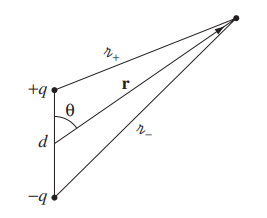
\includegraphics[width=6cm]{Electrodynamics/images/fig3.26.PNG}
\end{center}
Here, note that
\[V(\vec{r})=\frac{q}{4\pi\varepsilon_0}\left(\frac{1}{\scr_+}-\frac{1}{\scr_-}\right).\]
Note that from the law of cosines,
\[\scr_\pm^2=r^2+\left(\frac{d}{2}\right)^2\mp rd\cos\theta=r^2\left(1\mp \frac{d}{r}\cos\theta+\frac{d^2}{4r^2}\right).\]
Since we are interested in the regime $r\gg d$, the third term is negligible, so
\[\frac{1}{\scr_\pm}\approx \frac{1}{r}\left(1\mp \frac{d}{r}\cos\theta\right)^{-1/2}\approx \frac{1}{r}\left(1\pm\frac{d}{2r}\cos\theta\right).\]
Thus,
\[\boxed{V(\vec{r})\approx \frac{qd\cos\theta}{4\pi\varepsilon_0r^2}\qquad (r\gg d)}.\]
\end{proof}

Therefore, the potential of a dipole falls off with $1/r^2$ for large $r$. It makes sense that this falls off more rapidly than a point charge. Further, if we put two opposite dipoles together, we get a \vocab{quadrupole}, and it turns out that this potential falls off with $1/r^3$. We can then place two opposite quadrupoles together to form an \vocab{octopole}, whose potential falls off with $1/r^4$. This is summarized in the following figure:

\begin{center}
    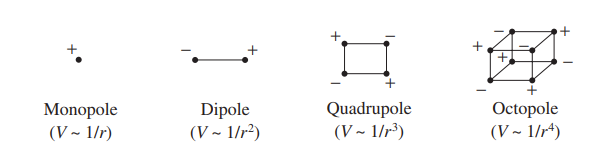
\includegraphics[width=10cm]{Electrodynamics/images/fig3.27.PNG}
\end{center}

Now, let's try to develop this theory for a general charge distribution $\rho$. The necessary variables are defined in the diagram below:

\begin{center}
    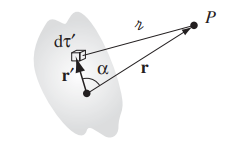
\includegraphics[width=6cm]{Electrodynamics/images/fig3.28.PNG}
\end{center}

Recall that
\[V(\vec{r})=\frac{1}{4\pi\varepsilon_0}\iiint_{\mathbb{R}^3}\frac{\rho(\vec{r'})}{\scr}d\tau'.\]
Using the law of cosines, we have
\[\scr^2=r^2+(r')^2-2rr'\cos\alpha=r^2\left[1+\left(\frac{r'}{r}\right)^2-2\left(\frac{r'}{r}\right)\cos\alpha\right].\]
If we define 
\[\epsilon:=\frac{r'}{r}\left(\frac{r'}{r}-2\cos\alpha\right),\]
then we can Taylor expand
\[\frac{1}{\scr}=\frac{1}{r}(1+\epsilon)^{-1/2}=\frac{1}{r}\left(1-\frac{1}{2}\epsilon+\frac{3}{8}\epsilon^2-\frac{5}{16}\epsilon^3+\cdots\right),\]
and substituting $\epsilon$ gives
\[\frac{1}{\scr}=\frac{1}{r}\left[1+\left(\frac{r'}{r}\right)(\cos\alpha)+\left(\frac{r'}{r}\right)^2\left(\frac{3\cos^2\alpha-1}{2}\right)+\left(\frac{r'}{r}\right)^3\left(\frac{5\cos^3\alpha-3\cos\alpha}{2}\right)\right].\]
Oh, look! The Legendre polynomials have showed up again! This is an alternative way to the Rodrigues' Formula to define the polynomials, where $1/\scr$ is a \textit{generating function} for the Legendre polynomials.
\[\frac{1}{\scr}=\frac{1}{r}\sum_{n=0}^\infty \left(\frac{r'}{r}\right)^nP_n(\cos\alpha).\]
Substituting this back into our formula for the potential gives
\[\boxed{V(\vec{r})=\frac{1}{4\pi\varepsilon_0}\sum_{n=0}^\infty \frac{1}{r^{n+1}}\iiint_{\mathbb{R}^3}(r')^nP_n(\cos\alpha)\rho(\vec{r'})d\tau'}.\]
This is the \vocab{multipole expansion} that we're searching for; it can be written explicitly as
\begin{align*}
V(\vec{r})=\frac{1}{4\pi\varepsilon_0}&\left[\frac{1}{r}\iiint \rho(\vec{r'})d\tau'+\frac{1}{r^2}\iiint r'\cos\alpha \rho(\vec{r'})d\tau'\right.\\
&\left.+\frac{1}{r^3}\iiint(r')^2\left(\frac{3}{2}\cos^2\alpha-\frac{1}{2}\right)\rho(\vec{r'})d\tau'+\cdots\right].
\end{align*}
Note that the first term is precisely $\frac{Q}{4\pi\varepsilon_0r}$ (as the integral of all the volume charge density should be exactly $Q$), what we would expect from a point charge. You can further check that the next term matches with $\frac{qd\cos\theta}{4\pi\varepsilon_0r^2}$ from the dipole moment above. The third is quadrupole, falling off with $1/r^3$; the fourth is octople, falling off with $1/r^4$; and so on.

\begin{remark}
If you're interested in the potential along the $z$-axis (so reorient your coordinate system so that $\vec{r}$ is pointing along the $z$-axis), then $\alpha$ is the usual polar angle $\theta$. 
\end{remark}

This multipole expansion is useful primarily as an approximation scheme, where you add more terms as more precision is needed.

\subsection{The Monopole and Dipole Terms}

At large $r$, the multipole expansion is dominated by the monopole term (as expected):
\[V_{\text{mon}}(\vec{r})=\frac{1}{4\pi\varepsilon_0}\frac{Q}{r},\]
where $Q=\iiint \rho d\tau$ is the total charge of the configuration. Of course, for the particular configuration of a single point charge at the origin, $V_{\text{mon}}$ is the \textit{exact} potential.

If the total charge is zero, this term vanishes, and the multipole expansion is dominated by the dipole term:
\[V_{\text{dip}}(\vec{r})=\frac{1}{4\pi\varepsilon_0}\frac{1}{r^2}\iiint_{\mathbb{R}^3}r'\cos\alpha \rho(\vec{r'})d\tau'.\]
Since $\alpha$ is the angle between $\vec{r}$ and $\vec{r'}$, we can write this more succinctly as
\[V_{\text{dip}}(\vec{r})=\frac{1}{4\pi\varepsilon_0}\frac{1}{r^2}\hat{r}\cdot\iiint_{\mathbb{R}^3}\vec{r'}\rho(\vec{r'})d\tau'.\]

\begin{definition}
The integral here (which luckily no longer depends on $\vec{r}$, since we removed the $\cos\alpha)$, is known as the \vocab{dipole moment} of the distribution:
\[\vec{p}:=\iiint_{\RR^3}\vec{r'}\rho(\vec{r'})d\tau'.\]
\end{definition}

With this definition, the dipole contribution simplifies to
\[V_{\text{dip}}(\vec{r})=\frac{1}{4\pi\varepsilon_0}\frac{\vec{p}\cdot\hat{r}}{r^2}.\]
The dipole moment is determined by the geometry (size, shape, and density) of the charge distribution. For a collection of $n$ point charges $q_i$, the dipole moment is simply
\[\vec{p}=\sum_{i=1}^n q_i\vec{r_i'}.\]
Therefore, for a physical dipole (as in Example \ref{physelecdip}), we have
\[\vec{p}=q\vec{r_+'}-q\vec{r_-'}=q\vec{d},\]
where $\vec{d}$ is the vector of length $d$ from the negative charge to the positive one.

Unlike the monopole, however, this is only the \textit{approximate} potential of the physical dipole, when $r$ is large (or $d$ is small). 

\begin{definition}
A \vocab{perfect dipole} is a physical dipole under the limit $d\to 0$, $q\to \infty$, while keeping the dipole moment $qd=p$ fixed. A perfect dipole's potential is exactly $V_{\text{dip}}$.
\end{definition}

Dipole moments are vectors, and they add like vectors. So given two dipoles with moments $\vec{p}_1$ and $\vec{p}_2$, the total dipole moment is $\vec{p}_1+\vec{p}_2$. Hence, the construction of the quadrupole: by arranging two opposite dipoles next to each other, the dipole moment is zero, so the potential is dominated by the quadrupole term in the multipole expansion.

\subsection{Origin of Coordinates in Multipole Expansion}

A point charge at the origin is a pure monopole. However, if it's off from the origin, it's no longer a pure monopole! For instance, a charge $q$ at $(0,d,0)$ has dipole moment $\vec{p}=qd\hat{y}$.

After all, the exact potential is $\frac{1}{4\pi\varepsilon_0}\frac{q}{\scr}$, not over $\frac{1}{4\pi\varepsilon_0}\frac{q}{r}$ (this is why we need to expand $1/\scr$ as a generating function anyway, to get all the Legendre polynomials/higher order terms).

Note, however, that moving the origin doesn't change the \vocab{monopole moment} $Q$ (or even the monopole term), it's just that the higher poles start to appear. In a similar way, movign the origin affects the dipole moment as well (and the higher pole terms). However, there is a special exception:

\begin{claim}
If the total charge is zero, then the dipole moment is independent of the choice of origin.
\end{claim}

\begin{proof}
If we displace the origin by an amount $\vec{a}$, then the new dipole moment is
\begin{align*}
\vec{p}_{\text{new}}&=\iiint \vec{r'}_{\text{new}}\rho(\vec{r'})d\tau'\\
&=\iiint (\vec{r'}-\vec{a})\rho(\vec{r'})d\tau'\\
&=\iiint \vec{r'}\rho(\vec{r'})d\tau'-\vec{a}\iiint\rho(\vec{r'})d\tau'\\
&=\vec{p}-Q\vec{a}.
\end{align*}
Therefore, if $Q=0$, then $\vec{p}_{\text{new}}=\vec{p}$.
\end{proof}

So if someone asks you for the dipole moment of configuration (a) below, you can confidently say $q\vec{d}$. But if someone asks you for the dipole moment of configuration (b) below, you should respond ``with respect to \textit{what origin}?"

\subsection{The Electric Field of a Dipole}

Let's use the potential to calculate the electric field of a perfect dipole. Change coordinates so that $\vec{p}$ is at the origin and pointing in the $z$ direction, then 
\[V_{\text{dip}}(r,\theta)=\frac{1}{4\pi\varepsilon_0}\frac{\vec{p}\cdot \hat{r}}{r^2}=\frac{p\cos\theta}{4\pi\varepsilon_0r^2}.\]
Now we take the negative gradient of $V$ to get the electric field $\vec{E}$:
\begin{align*}
    E_r&=-\frac{\partial V}{\partial r}=\frac{p\cos\theta}{2\pi\varepsilon_0r^3}\\
    E_\theta&=-\frac{1}{r}\frac{\partial V}{\partial\theta}=\frac{p\sin\theta}{4\pi\varepsilon_0 r^3}\\
    E_\varphi&=-\frac{1}{r\sin\theta}\frac{\partial V}{\partial \varphi}=0
\end{align*}
Hence,
\[\vec{E}_{\text{dip}}(r,\theta)=\frac{p}{4\pi\varepsilon_0r^3}(2\cos\theta \cdot\hat{r}+\sin\theta\cdot\hat{\theta}).\]
This makes explicit reference to a particular coordinate system (spherical), and assumes a particular orientation for $\vec{p}$ (along the $z$-axis). Note that the dipole electric field falls off with the inverse \textit{cube} of $r$ (after all, the monopole field falls of with the inverse \textit{square}). This makes sense since the gradient simply introduces another factor of $1/r$ into the potential drop offs. 

Below is a picture of a pure dipole electric field and a physical dipole electric field. Note how for $r\gg d$, they pretty much agree.

\begin{center}
    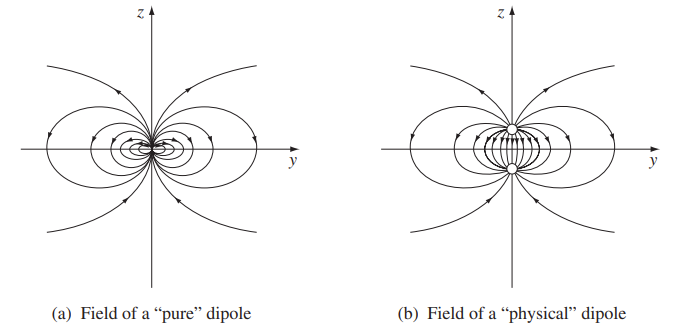
\includegraphics[width=12cm]{Electrodynamics/images/fig3.37.PNG}
\end{center}